\documentclass[12pt]{report}
\usepackage[spanish]{babel}
\usepackage[utf8]{inputenc}
\usepackage{amsmath}
\usepackage{amssymb}
\usepackage{amsthm}
\usepackage{graphics}
\usepackage{subfigure}
\usepackage{lipsum}
\usepackage{array}
\usepackage{multicol}
\usepackage{enumerate}
\usepackage[framemethod=TikZ]{mdframed}
\usepackage[a4paper, margin = 1.5cm]{geometry}
\usepackage{tikz}
\usepackage{pgffor}
\usepackage{ifthen}
\usepackage{listings}
\usepackage{hyperref}
\usepackage{xcolor}
\usepackage{enumitem}
\usepackage{mathdots}
\usepackage{bbm}

%Gestión de Hipervínculos

\hypersetup{
    colorlinks=true,
    linkcolor=black,
    filecolor=magenta,      
    urlcolor=cyan
}

%Gestión de Código de Programación

\definecolor{listing-background}{HTML}{F7F7F7}
\definecolor{listing-rule}{HTML}{B3B2B3}
\definecolor{listing-numbers}{HTML}{B3B2B3}
\definecolor{listing-text-color}{HTML}{000000}
\definecolor{listing-keyword}{HTML}{435489}
\definecolor{listing-keyword-2}{HTML}{1284CA} % additional keywords
\definecolor{listing-keyword-3}{HTML}{9137CB} % additional keywords
\definecolor{listing-identifier}{HTML}{435489}
\definecolor{listing-string}{HTML}{00999A}
\definecolor{listing-comment}{HTML}{8E8E8E}

\lstdefinestyle{myStyle}{
    language         = java,
    alsolanguage     = scala,
    numbers          = left,
    xleftmargin      = 2.7em,
    framexleftmargin = 2.5em,
    backgroundcolor  = \color{gray!15},
    basicstyle       = \color{listing-text-color}\linespread{1.0}\ttfamily,
    breaklines       = true,
    frameshape       = {RYR}{Y}{Y}{RYR},
    rulecolor        = \color{black},
    tabsize          = 2,
    numberstyle      = \color{listing-numbers}\linespread{1.0}\small\ttfamily,
    aboveskip        = 1.0em,
    belowskip        = 0.1em,
    abovecaptionskip = 0em,
    belowcaptionskip = 1.0em,
    keywordstyle     = {\color{listing-keyword}\bfseries},
    keywordstyle     = {[2]\color{listing-keyword-2}\bfseries},
    keywordstyle     = {[3]\color{listing-keyword-3}\bfseries\itshape},
    sensitive        = true,
    identifierstyle  = \color{listing-identifier},
    commentstyle     = \color{listing-comment},
    stringstyle      = \color{listing-string},
    showstringspaces = false,
}

\lstset{style = myStyle}

%Gestión de Marca de Agua

\newcounter{it}
\newcommand*\watermarktext[1]{\begin{tabular}{c}
    \setcounter{it}{1}%
    \whiledo{\theit<100}{%
    \foreach \col in {0,...,15}{#1\ \ } \\ \\ \\
    \stepcounter{it}%
    }
    \end{tabular}
    }

\AddToHook{shipout/foreground}{
    \begin{tikzpicture}[remember picture,overlay, every text node part/.style={align=center}]
        \node[rectangle,black,rotate=30,scale=2,opacity=0.04] at (current page.center) {\watermarktext{Cristo Daniel Alvarado ESFM\quad}};
  \end{tikzpicture}
}

%Redefinición de comandos

\def\proof{\paragraph{Demostración:\\}}
\def\endproof{\hfill$\blacksquare$}

\def\sol{\paragraph{Solución:\\}}
\def\endsol{\hfill$\square$}

%Definición de ambientes

\newtheoremstyle{largebreak}
  {}% use the default space above
  {}% use the default space below
  {\normalfont}% body font
  {}% indent (0pt)
  {\bfseries}% header font
  {}% punctuation
  {\newline}% break after header
  {}% header spec

\theoremstyle{largebreak}

\newmdtheoremenv[
    leftmargin=0em,
    rightmargin=0em,
    innertopmargin=0pt,
    innerbottommargin=5pt,
    hidealllines = true,
    roundcorner = 5pt,
    backgroundcolor = gray!60!red!30
]{exa}{Ejemplo}[section]

\newmdtheoremenv[
    leftmargin=0em,
    rightmargin=0em,
    innertopmargin=0pt,
    innerbottommargin=5pt,
    hidealllines = true,
    roundcorner = 5pt,
    backgroundcolor = gray!50!blue!30
]{obs}{Observación}[section]

\newmdtheoremenv[
    leftmargin=0em,
    rightmargin=0em,
    innertopmargin=0pt,
    innerbottommargin=5pt,
    rightline = false,
    leftline = false
]{theor}{Teorema}[section]

\newmdtheoremenv[
    leftmargin=0em,
    rightmargin=0em,
    innertopmargin=0pt,
    innerbottommargin=5pt,
    rightline = false,
    leftline = false
]{propo}{Proposición}[section]

\newmdtheoremenv[
    leftmargin=0em,
    rightmargin=0em,
    innertopmargin=0pt,
    innerbottommargin=5pt,
    rightline = false,
    leftline = false
]{cor}{Corolario}[section]

\newmdtheoremenv[
    leftmargin=0em,
    rightmargin=0em,
    innertopmargin=0pt,
    innerbottommargin=5pt,
    rightline = false,
    leftline = false
]{lema}{Lema}[section]

\newmdtheoremenv[
    leftmargin=0em,
    rightmargin=0em,
    innertopmargin=0pt,
    innerbottommargin=5pt,
    roundcorner=5pt,
    backgroundcolor = gray!30,
    hidealllines = true
]{mydef}{Definición}[section]

\newmdtheoremenv[
    leftmargin=0em,
    rightmargin=0em,
    innertopmargin=0pt,
    innerbottommargin=5pt,
    roundcorner=5pt
]{excer}{Ejercicio}[section]

%Definición de nuevas funciones

\newcommand\abs[1]{\ensuremath{\left|#1\right|}}
\newcommand\divides{\ensuremath{\bigm|}}
\newcommand\cf[3]{\ensuremath{#1:#2\rightarrow#3}}
\newcommand\contradiction{\ensuremath{\#_c}}
\newcommand\natint[1]{\ensuremath{\left[\big|#1\big|\right]}}
\newcommand{\dom}[1]{\textup{dom}\left(#1 \right)}
\newcommand{\bbm}[1]{\ensuremath{\mathbbm{#1}}}

\begin{document}
    \setlength{\parskip}{5pt} % Añade 5 puntos de espacio entre párrafos
    \setlength{\parindent}{12pt} % Pone la sangría como me gusta
    \title{Curso de Lógica Matemática
    
    Teoría de la Computabilidad}
    \author{Cristo Daniel Alvarado}
    \maketitle

    \tableofcontents %Con este comando se genera el índice general del libro

    \newpage

    \setcounter{chapter}{2}

    \chapter{Conjuntos y Funciones computables}

    Todo de lo que se va a tratar esta parte es de: ¿Cómo formalizar la noción de \textit{procedimiento mecánico, efectivo} o \textit{sistemático}? Con esto nos referimos a:
    \begin{itemize}
        \item Tener un número finito de instrucciones.
        \item Terminar el procedimiento en un número finito de pasos.
        \item Usar únicamente \textit{papel y lápiz}.
        \item No requiere razonamiento, solo se siguen reglas.
    \end{itemize}

    Básicamente se pretendía que dada una fórmula, encontrar un algoritmo que nos diga si esa fórmula es verdadera o falsa. Básicamente se pretendía formalizar las demostraciones para ver lo que nosotros podemos demostrar únicamente usando los axiomas.

    Turing y Alonzo Church eventualmente se hicieron preguntas en la misma dirección. En la Tesis de Church-Turing se probó que estas tres preguntas en realidad se reducen a un mismo problema.

    \section{Máquinas de Turing}

    \begin{mydef}
        Una \textbf{máquina de Turing} consta de:
        \begin{itemize}
            \item Un \textit{alfabeto}, un conjunto finito $L$.
            \item Un conjunto finito $S$ de \textit{estados}.
            \item Una función parcial $\cf{T}{L^*\times S}{L^*\times S\times\left\{<,-,> \right\}}$ llamada \textit{función de transición}.
        \end{itemize}
        donde $L^*=L\cup\left\{* \right\}$.
    \end{mydef}

    Intuitivamente, uno debe imaginar que esto es una especie de \textit{computadora rudimentaria}. Generalmente esto se conceptualiza como una cinta.

    \begin{center}
        \label{Turing1}
        \begin{figure}
            \begin{center}
                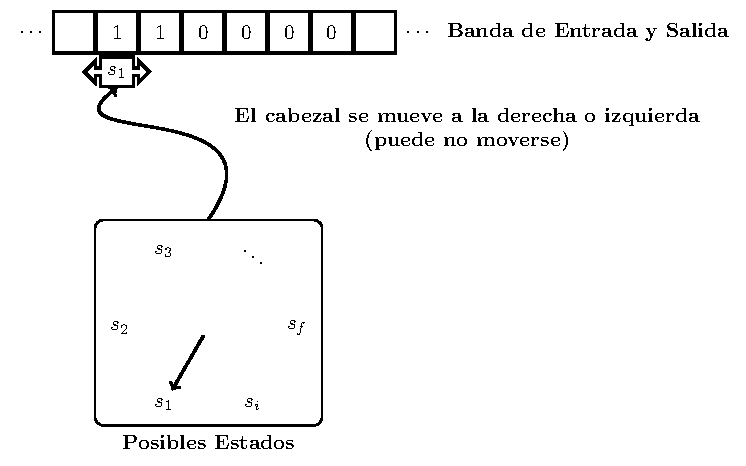
\includegraphics[scale=1]{images/fig_1.pdf}
            \end{center}
            \caption{Ejemplo de Máquina de Turing}
        \end{figure}
    \end{center}

   El cabezal $c$ puede moverse a la derecha, izquierda o no moverse, dependiendo del estado en el que esté. En la Figura \ref{Turing1} se muestra que el hay al menos 5 diferentes estados, desde el estado inicial ($s_i$) hasta el final ($s_f$). Dependiendo de la entrada, la función $T$ nos dirá lo que hará el cabezal, si cambia un elemento de la banda, si se mueve o si cambia de estado (o todas a la vez).

   En este ejemplo, el alfabeto sería $L=\left\{0,1 \right\}$, el conjunto de estados es $S=\left\{s_i,s_1,...,s_f \right\}$ y la función sería representada por lo que sea que haga el cabezal.

    \begin{exa}
        Considere $L=\left\{1 \right\}$, $S=\left\{s_i,s_1,s_2 \right\}$ y,
        \begin{equation*}
            T=\left\{(s_i,*,s_1,*,>),(s_i,1,s_1,1,>),(s_1,1,s_1,1,>),(s_1,1,s_2,1,-) \right\}
        \end{equation*}
        La cinta se ve más o menos así:

    \end{exa}

    Para los siguientes ejercicios, ir a la página: \href{https://turingmachinesimulator.com/}{Simulador Máquina de Turing}.

    \begin{excer}
        Codifique una máquina de Turing que sume 1 a un número dado en binario.
    \end{excer}

    \begin{lstlisting}
        name: Sumar uno en unario
        init: s0
        accept: sf

        
        // Funciones de Transicion

        s0,_
        s0,_,>

        s0,1
        s1,1,-

        s0,0
        s1,0,-

        s1,1
        s1,0,>

        s1,0
        s1,1,>

        s1,_
        sf,_,-

        // < = left
        // > = right
        // - = hold
        // use _ for blank cells

        // States and symbols are case-sensitive

        // Load your code and click COMPILE.
        //  or load an example (top-right).
    \end{lstlisting}

    \begin{excer}
        Codifique una máquina de Turing que dada un número en binario, invierta su orientación, es decir, si la cadena es $(a_1,...,a_n)$, que la máquina de Turing la convierta en $(a_n,...,a_1)$. 
    \end{excer}

    \begin{lstlisting}
        name: invertirCadena
        init: s0
        accept: s1,sf,l,c,u
        
        //esto para que se empiece a mover
        s0,_
        s0,_,>
        
        s0,0
        x,0,<
        
        s0,1
        x,1,<
        
        x,_
        s1,2,>
        
        s1,0
        s1,0,>
        
        s1,1
        s1,1,>
        
        //logica cuando encuentre cosas
        
        s1,_
        s2,_,<
        
        s2,_
        s2,_,<
        
        s2,0
        c00,_,>
        
        s2,1
        u00,_,>
        
        //mueve cosas al inicio
        
        c00,_
        m,0,<
        
        u00,_
        m,1,<
        
        //ya en ciclo
        
        //mueve derecha
        
        m,_
        l,_,<
        
        l,_
        l,_,<
        
        l,0
        c0,_,>
        
        l,1
        u0,_,>
        
        c0,_
        c0,_,>
        
        //mueve izquierda
        
        u0,_
        u0,_,>
        
        c0,0
        c1,0,>
        
        c0,1
        c1,1,>
        
        u0,0
        u1,0,>
        
        u0,1
        u1,1,>
        
        c1,0
        c1,0,>
        
        c1,1
        c1,1,>
        
        u1,0
        u1,0,>
        
        u1,1
        u1,1,>
        
        c1,_
        m,0,<
        
        u1,_
        m,1,<
        
        m,0
        m,0,<
        
        m,1
        m,1,<
        
        l,2
        sf,_,>
        
        sf,_
        sf,_,>
        
        sf,0
        sff,0,-
        
        sf,1
        sff,1,-        
    \end{lstlisting}

    \begin{mydef}
        Una función $f$ es \textbf{computable} si:
        \begin{enumerate}[label = \textit{(\arabic*)}]
            \item $\dom{f}\subseteq\mathbb{N}$.
            \item Existe un algoritmo tal que para cada $n\in\mathbb{N}$, el algoritmo al correrse con $n$ como argumento, se detiene en tiempo finito si y sólo si $n\in\dom{f}$ y en tal caso arroja $f(n)$ como salida. 
        \end{enumerate}
    \end{mydef}

    ¿Qué es un algoritmo? Resulta que hay muchas formas de definirlo, sin embargo, nosotros adoptaremos la siguiente definición:

    \begin{mydef}
        Un \textbf{algoritmo} lo interpretaremos como una máquina de Turing.
    \end{mydef}

    \begin{obs}
        Un algoritmo también puede verse como un código en C, C++, Python o \LaTeX (usando las librerías adecuadas).
    \end{obs}

    En la Tesis de Church-Turing, cualquier noción es equivalente.

    \begin{obs}
        De ahora en adelante consideraremos a los naturales con el 0.
    \end{obs}

    \begin{exa}
        La función $\cf{f}{\mathbb{N}\setminus\left\{0,1\right\}}{\mathbb{N}}$ tal que $n\mapsto\min\left\{p\in\mathbb{N}\Big|p\textup{ es primo y }p\divides n \right\}$ es computable.
    \end{exa}

    \begin{proof}
        Se tiene el siguiente algoritmo:
        \begin{lstlisting}
int f(int n){
    for(int k = 2;n % k != 0;k++) return k;
}
        \end{lstlisting}
    \end{proof}

    \begin{exa}
        Considere la función $\cf{g}{\left\{n^2\Big|n\in\mathbb{N} \right\}}{\mathbb{N}}$ dada por $n^2\mapsto n$. Esta función es computable.
    \end{exa}

    \begin{proof}
        Se tiene el siguiente algoritmo:
        \begin{lstlisting}
int g(int m){
    for(int k = 0;k*k != m;k++) return k;
}
        \end{lstlisting}
    \end{proof}

    \begin{exa}
        La función $\cf{+}{\mathbb{N}\times\mathbb{N}}{\mathbb{N}}$ es computable.
    \end{exa}

    \begin{proof}
        Recordemos que existe una biyección entre $\mathbb{N}\times\mathbb{N}$ y $\mathbb{N}$ dada por:
        \begin{equation*}
            (k,l)\mapsto 2^k(2l+1)
        \end{equation*}
        por lo cual, podemos ver a la función suma como una función de $\mathbb{N}$ en $\mathbb{N}$.
    \end{proof}

    \begin{obs}
        Podemos ir más allá en el ejemplo anterior, podemos generalizar la idea anterior usando conjuntos que puedan ser representados mediante números naturales (recuerde la enumeración de Gödel).
    \end{obs}

    Veremos más ejemplos que nos ayudarán más adelante a hacer cosas más complejas:

    \begin{itemize}
        \item La función sucesor (se vió en un ejercicio anterior).
        \item Cualquier función constante.
        \item La $i$-ésima proyección de una $k$-tupla.
    \end{itemize}
    \begin{lstlisting}
int p_2(int a, int b, int c){
    return b;
}
    \end{lstlisting}
    este ejemplo anterior es la 2-ésima proyección de una 3-tupla.

    \begin{exa}
        La función exponencial: $(a,b)\mapsto a^{b}$ es computable.
    \end{exa}

    \begin{proof}
        En efecto, se tiene el siguiente algoritmo:
        \begin{lstlisting}
int exp(int a, int b){
    if(b==0){
        return 1;
    }
    else return a*exp(a,b-1);
}
        \end{lstlisting}
    \end{proof}

    \begin{exa}
        La función factorial $n\mapsto n!$ es computable.
    \end{exa}

    \begin{proof}
        En efecto, se tiene el siguiente algoritmo:
        \begin{lstlisting}
int fact(int n){
    if(n==0) return 1;
    else return n*fact(n-1);
}
        \end{lstlisting}
    \end{proof}

    \begin{exa}
        Las funciones máximo y mínimo son computables.
    \end{exa}

    \begin{exa}
        El algoritmo de la división es computable.
    \end{exa}

    \begin{proof}
        En efecto, se tiene el siguiente algoritmo:
        \begin{lstlisting}
int div(int a, int b){
    for(int i=1; i*b<=a;i++){} //se queda y acaba si es que se puede dividir
    q = i-1;
    r = a-b*q;
    return exp(2,q)*(2*r-1); //codificamos de esta manera la salida del programa
}
        \end{lstlisting}
    \end{proof}

    \begin{obs}
        Cuando coloquemos $\cf{f}{;A}{B}$, entenderemos que $\dom{f}\subseteq A$, es decir que $f$ es una función parcial.
    \end{obs}

    \begin{theor}
        Sea $\cf{f}{;\mathbb{N}^k}{\mathbb{N}}$ una función computable, y sean $\cf{g_1,...,g_k}{;\mathbb{N}}{\mathbb{N}}$ funciones computables. Entonces:
        \begin{enumerate}[label = \textit{(\arabic*)}]
            \item La función $\cf{h_1}{;\mathbb{N}}{\mathbb{N}}$ dada por: $h_1(x)=f(g_1(x),\cdots,g_k(x))$ es computable.
            \item La función $\cf{h_2}{;\mathbb{N}^{ k-1}}{\mathbb{N}}$ dada por:
            \begin{equation*}
                h_2(x_2,\cdots,x_k)=(\mu x)(f(x,x_2,\cdots,x_k)=0)
            \end{equation*}
            donde la función $\mu x$ es el mínimo de $x$ tal que lo de adentro se hace 0, siendo $f$ tal que para todo $i\leq x$, $f(i,x_2,...,x_k)$ está bien definido, también es computable.
        \end{enumerate}
    \end{theor}

    \begin{proof}
        De \textit{(1)}: Considere el algoritmo:
        \begin{lstlisting}
int h_1(int x){
    int y_1 = g_1(x);
    int y_2 = g_2(x);
    ...
    int y_k = g_k(x);
    return f(y_1,...,y_k);
}
        \end{lstlisting}
    \end{proof}
    es una función computable, ya que si no puede calcular algún valor, se queda atorado.

    De \textit{(2)}: Considere el algoritmo:
    \begin{lstlisting}
        int h_2(int x_2,...,int x_k){
            for(int x=0; f(x,x_2,...,x_k)!=0;x++) return x;
        }
    \end{lstlisting}
    es de una función computable.

    \begin{mydef}
        Una función computable $\cf{f}{;\mathbb{N}^k}{\mathbb{N}}$ es \textbf{total}, si $\dom{f}=\mathbb{N}^k$. En computabilidad esto se denota por:
        \begin{equation*}
            (\forall x_1,...,x_k)(f(x_1,...,x_k)\downarrow)
        \end{equation*}
        esto es, que para cualquier entrada $f$ está bien definida.
    \end{mydef}

    \begin{obs}
        En el teorema anterior, siempre se puede hacer (2) si la función $f$ es total.
    \end{obs}

    \begin{excer}
        Codifique una máquina de Turing que sume dos números en binario.
    \end{excer}

    \begin{lstlisting}
name: suma_numeros_binario
init: s0
accept: sf

s0,_
s0,_,>

s0,0
s1,0,>

s1,0
s1,0,>

s0,1
s1,1,>

s1,1
s1,1,>

//operaciones de suma

//el estado s_s0 nos dice que va a empezar a contar el otro numero
//el estado s_s1 nos dice que encontro un numero positivo para sumar

s1,+
s_s0,+,>

s_s0,0
s_s0,0,>

s_s0,1
s_s1,1,>

s_s1,1
s_s1,1,>

s_s1,0
s_s1,0,>

//llego al final de la cadena

s_s1,_
sr0,_,<

sr0,1
srf,0,>

sr0,0
sr0,0,<

srf,0
srf,1,>

srf,_
ss0,_,<

//ss es que ahora le va sumar uno a la cadena de la izquierda

ss0,0
ss0,0,<

ss0,1
ss0,1,<

ss0,+
ss1,+,<

ss1,0
s1,1,>

ss1,1
ss1,0,<

ss1,_
s1,1,>

//cuando no haya nada por sumar, simplemente se detiene

s_s0,_
sf0,_,<

sf0,0
sf0,_,<

sf0,+
sf,_,-

// < = left
// > = right
// - = hold
// use underscore for blank cells

//States and symbols are case-sensitive

//Load your code and click COMPILE.
//or load an example (top-right).
    \end{lstlisting}

    \begin{excer}
        Codifique una máquina de Turing que sume dos números en binario.
    \end{excer}

\begin{lstlisting}
name: resta_numeros_1
init: s0
accept: sf

s0,_
s0,_,>

s0,0
s1,0,>

s1,0
s1,0,>

s0,1
s1,1,>

s1,1
s1,1,>

//operaciones de resta

//sr0 es estado resta inicial

//srf es estado resta final

s1,_
sr0,_,<

sr0,1
srf,0,>

sr0,0
sr0,0,<

srf,0
srf,1,>

srf,_
sf,_,-

// < = left
// > = right
// - = hold
// use underscore for blank cells

//States and symbols are case-sensitive

//Load your code and click COMPILE.
//or load an example (top-right).
\end{lstlisting}

\begin{excer}
    Dada una cadena en binario, escribir un programa que haga una copia de la misma.
\end{excer}

\begin{lstlisting}
name: copiar_cadena
init: s0
accept: sf

//se empieza a mover y marca el inicio de la cadena

s0,_
s0,_,>

s0,0
s1,0,<

s2,0
s2,0,>

s0,1
s1,1,<

s2,1
s2,1,>

s1,_
s2,|,>

s2,0
s2,0,>

s2,1
s2,1,>

//coloca el inicio de la copia de la cadena

s2,_
sd,c,<

sd,0
sd,0,<

sd,1
sd,1,<

sd,2
sd,2,<

sd,3
sd,3,<

sd,c
sd,c,<

sd,|
sdp,|,>

//deteccion de si es 0 o 1

sdp,0
sdp0,2,>

sdp,1
sdp1,3,>

sdp,2
sdp,2,>

sdp,3
sdp,3,>

//movimiento a la derecha para colocar 0 o 1

sdp0,0
sdp0,0,>

sdp0,1
sdp0,1,>

sdp1,0
sdp1,0,>

sdp1,1
sdp1,1,>

//detecta la copia

sdp0,c
sdp0,c,>

sdp1,c
sdp1,c,>

sdp0,_
sd,0,<

sdp1,_
sd,1,<

//detecta que ya debe terminar

sdp,c
scam,c,<

scam,2
scam,0,<

scam,3
scam,1,<

scam,|
sf,_,-
\end{lstlisting}

\begin{excer}
    Programar una máquina de Turing que haga el producto de dos números. 
\end{excer}

\begin{lstlisting}
name: producto_numeros
init: p0
accept: pf

//input: [n]_2*[m]_2

//empieza el movimiento

p0,_
p0,_,>

p0,0
p1,0,<

p0,1
p1,1,<

p1,_
p2,|,>

p2,0
p2,0,>

p2,1
p2,1,>

p2,*
p2,*,>

//llego al final de la cadena

p2,_
sd,c,<

//PARTE PRIMERA COPIA

sd,0
sd,0,<

sd,1
sd,1,<

sd,2
sd,2,<

sd,3
sd,3,<

sd,*
sd,*,<

sd,c
sd,c,<

sd,|
sdp,|,>

//deteccion de si es 0 o 1

sdp,0
sdp0,2,>

sdp,1
sdp1,3,>

sdp,2
sdp,2,>

sdp,3
sdp,3,>

sdp,c
sdp,c,>

//movimiento a la derecha para colocar 0 o 1

sdp0,0
sdp0,0,>

sdp0,1
sdp0,1,>

sdp1,0
sdp1,0,>

sdp1,1
sdp1,1,>

//detecta la copia

sdp0,*
sdp0,*,>

sdp1,*
sdp1,*,>

sdp0,c
sdp0,c,>

sdp1,c
sdp1,c,>

sdp0,_
sd,0,<

sdp1,_
sd,1,<

//detecta que ya debe terminar y elimina los cambios que hizo

sdp,*
scam,*,<

scam,2
scam,0,<

scam,3
scam,1,<

scam,|
sf,_,>

//segunda copia

sf,0
sf,0,>

sf,1
sf,1,>

sf,*
sf,*,>

sf,c
sf,c,>

//ahora, hace la segunda copia

//coloca el inicio de la copia de la cadena

sf,_
rd,d,<

rd,0
rd,0,<

rd,1
rd,1,<

rd,2
rd,2,<

rd,3
rd,3,<

rd,d
rd,d,<

rd,c
rdp,c,>

//deteccion de si es 0 o 1

rdp,0
rdp0,2,>

rdp,1
rdp1,3,>

rdp,2
rdp,2,>

rdp,3
rdp,3,>

//movimiento a la derecha para colocar 0 o 1

rdp0,0
rdp0,0,>

rdp0,1
rdp0,1,>

rdp1,0
rdp1,0,>

rdp1,1
rdp1,1,>

//detecta la copia

rdp0,d
rdp0,d,>

rdp1,d
rdp1,d,>

rdp0,_
rd,0,<

rdp1,_
rd,1,<

//detecta que ya debe terminar

rdp,d
rcam,d,<

rcam,2
rcam,0,<

rcam,3
rcam,1,<

rcam,c
rf,c,<

rf,0
rf,0,<

rf,1
rf,1,<

rf,*
rf,*,<

//ahora ya puede empezar a sumar uno por uno

rf,_
rs,_,>

rs,0
rs,0,>

rs,1
rs,1,>

rs,*
rs,*,>

rs,c
rs,c,>

rs,d
rs,d,>

//hace la primera suma

rs,_
rsr,_,<

rsr,1
rss,0,>

rss,0
rss,1,>

rss,_
Rf,_,<

//en Rf

Rf,0
Rf,0,<

Rf,1
Rf,1,<

Rf,c
Rf,c,<

Rf,d
Rf,d,<

//ahora, si detecta el * es pq ahora tiene que sumar

Rf,*
estSum,*,<

estSum,0
estSumAcaba,1,>

estSum,_
estSumAcaba,1,>

estSum,1
estSum,0,<

//aqui acabo de sumar

rsr,0
RF,0,-

//se mueve para ahora sumar a la otra cadena    
    \end{lstlisting}

    \begin{mydef}
        Un conjunto $X$ es \textbf{computable}, si puede ser visto como input de elementos de $\mathbb{N}$, y su función característica es computable.
    \end{mydef}
    
    \begin{exa}
        Sea $\cf{F}{\mathbb{N}}{\mathbb{N}}$ la función:
        \begin{equation*}
            F(n)=\left\{
                \begin{array}{lcr}
                    1 & \textup{si} & \textup{conjetura Gölbach es verdadera.}\\
                    0 & \textup{ en } & \textup{caso contrario.}\\
                \end{array}
            \right.
        \end{equation*}
        esta función es computable.
    \end{exa}

    \begin{exa}
        La funcion $\cf{f}{\mathbb{N}}{\mathbb{N}}$ tal que:
        \begin{equation*}
            f(n)=\min\left\{p\Big|p>n\textup{ y tanto }p\textup{ como }p+2\textup{ son primos}\right\}
        \end{equation*}
        en efecto, se tiene el siguiente algoritmo de $f$:
    \end{exa}

    \begin{lstlisting}
int f(int n){
    for(int i=n+1; i no es primo || i+2 tampoco lo es; i++){
        return i;
    }
}
    \end{lstlisting}

    \section{Máquina Universal de Turing}

    En general, los input de mis algoritmos son $\mathbb{N}$, pero podemso también codificar parejas por medio de números naturales, por lo que realmente también podemos introducir tuplas de $\mathbb{N}^k$.

    \begin{obs}
        Una máquina de Turing es un conjunto finito $\left\{a_1,...,a_n \right\}$, donde $a_i=(s_{i_1},t_{i_2},s_{i_3},t_{i_4},l)$ con $l\in\left\{<,-,> \right\}$. Podemos hacer una codificación estas 6-tuplas:
        \begin{center}
            \begin{tabular}{l | c | r}
                0 & - & 0 \\
                1 & - & | \\
                2 & - & * \\
                3 & - & > \\
                $\vdots$ & - & $\vdots$ \\
            \end{tabular}
        \end{center}
        en este caso, codificamos elementos de $\left[\left\{0,1,*,<,>,-,s_1,...,s_n \right\}^k\right]^{<\aleph_0}$ (cadenas finitas de tuplas finitas). Lo que podemos hacer enotnces es codificar máquinas de Turing.
    \end{obs}

    \begin{theor}
        El conjunto
        \begin{equation*}
            \left\{x\in X\Big|x\textup{ es máquina de Turing} \right\}
        \end{equation*}
        y,
        \begin{equation*}
            \left\{n\in\mathbb{N}\Big|n\textup{ codifica una máquina de Turing} \right\}
        \end{equation*}
        son computables.
    \end{theor}

    \begin{proof}
        Ver simulador de máquina de Turing.
    \end{proof}
    
    \begin{mydef}
        Denotaremos la \textbf{máquina universal de Turing} por $\varphi$, donde
        \begin{equation*}
            \cf{\varphi}{;\mathbb{N}^2}{\mathbb{N}}
        \end{equation*}
        dada por $\varphi(e,n)$ es el resultado de correr la $e$-ésima máquina de Turing con input $n$.
    \end{mydef}

    \begin{obs}
        $\varphi$ es una función computable.
    \end{obs}

    Una forma de interpretar a $\varphi$ es el simulador de máquina de Turing, pues en este simulador introducimos una máquina de Turing y un input, así que nuestro código sería $e$ y el input sería $n$.
    
    \begin{mydef}
        La función $\cf{\varphi(e,-)}{\mathbb{N}}{\mathbb{N}}$ tal que $n\mapsto\varphi(e,n)$ es llamada la \textbf{$e$-ésima función computable}.
    \end{mydef}

    \begin{theor}[\textbf{Lema del Relleno}]
        Para cada función computable $f$, existen una infinidad de $e\in\mathbb{N}$ tales que $f=\varphi(e,-)$.
    \end{theor}

    Existen funciones que no son computables.

    \begin{obs}
        Como se pueden enumerar todas las funciones computables, el conjunto:
        \begin{equation*}
            \abs{\left\{\cf{f}{\mathbb{N}}{\mathbb{N}}\Big|f\textup{ es computable}\right\}}=\aleph_0
        \end{equation*}
        pero,
        \begin{equation*}
            \abs{\left\{\cf{f}{\mathbb{N}}{\mathbb{N}}\Big|f\textup{ es función} \right\}}=\aleph_1
        \end{equation*}
    \end{obs}

    \begin{exa}
        Se define la función \textbf{Busy Beaver}, $\cf{\sigma}{\mathbb{N}}{\mathbb{N}}$ dada por:
        \begin{equation*}
            \sigma(n)=\max\left\{\textup{output en unario de una máquina de Turing con }\leq n+1\textup{ estados e input }0 \right\}
        \end{equation*}
        de forma inmediata se tiene que $\sigma(0)=1$, ya que solo hay una máquina de Turing con un estado (el estado final), y el mayor output que puede hacer es 1.
    \end{exa}

    \begin{excer}
        Verifique que $\sigma(2)\geq4$.
    \end{excer}

    \begin{theor}
        Si $\cf{f}{\mathbb{N}}{\mathbb{N}}$ es cualquier función computable, entonces existe $N\in\mathbb{N}$ tal que para todo $n\geq N$ se cumple que $f(n)< \sigma(n)$. En particular, \textbf{$\sigma$ no es computable}.
    \end{theor}

    \begin{proof}
        Sea $f$ computable, entonces la función $\cf{g}{;\mathbb{N}}{\mathbb{N}}$ dada por:
        \begin{equation*}
            g(n)=\min\left\{f(2n),f(2n+1) \right\}+1
        \end{equation*}
        también es computable. Por lo tanto, existe alguna máquina de Turing $T$ que calcula a $g$ en unario. Sea $k$ el número de estados (además del estado inicial) de dicha máquina.

        Consideremos la función 
    \end{proof}

    \section{Conjuntos y Relaciones Computables}

    \begin{mydef}
        Un conjunto $X\subseteq\mathbb{N}$ es \textbf{computable} si su función característica $\chi_X$ es total computable.
    \end{mydef}

    \begin{exa}
        Los siguientes son conjuntos computables:
        \begin{enumerate}[label = \textit{(\arabic*)}]
            \item $\mathbb{N}$.
            \item $\emptyset$.
            \item $\left\{n\in\mathbb{N}\Big|n\textup{ es cuadrado perfecto} \right\}$.
            \item $\left\{p\in\mathbb{N}\Big|p\textup{ es primo} \right\}$.
            \item $\left\{(n,m)\in\mathbb{N}^2\Big|n\divides m \right\}$.
        \end{enumerate}
    \end{exa}

    \begin{sol}
        En efecto, se tienen los siguientes algoritmos de cada una de las funciones características de los conjuntos anteriores:
        \begin{lstlisting}
int uno(int n) return 1;

int dos(int n) return 0;

int tres(int n){
    for(int i=0; i*i<n;i++){
        if(i*i=n) return 1;
    }
    return 0;
}
        \end{lstlisting}
    \end{sol}

    \begin{propo}
        Sean $X,Y\subseteq\mathbb{N}$ conjuntos computables, entonces $X\cap Y$, $X\cup Y$ y $X\setminus Y$ son también computables (en otras palabras, el conjunto de conjuntos computables es un álgebra booleana).
    \end{propo}

    \begin{proof}
        Basta con ver que:
        \begin{itemize}
            \item $\chi_X(n)\chi_Y(n)=\chi_{ X\cap Y}(n)$.
            \item $\chi_{ X\cup Y}(n)=\max\left\{\chi_X(n),\chi_Y(n) \right\}$.
            \item $\chi_{ X\setminus Y}(n)=\max\left\{1-\chi_X(n),0 \right\}$.
        \end{itemize}
        para todo $n\in\mathbb{N}$.
    \end{proof}

    \begin{theor}
        El conjunto
        \begin{equation*}
            \left\{e\in\mathbb{N}\Big|\varphi(e,-)\textup{ es una función total} \right\}
        \end{equation*}
        no es computable.
    \end{theor}

    \begin{proof}
        En caso contrario, se tendría que la funcioń $h:n\mapsto n$-ésima máquina de Turing que induce una función total, también sería computable (ya que la característica detecta si una función computable es total o no, luego en particular existe una función que codifica a todas las funciones totales).

        Se sigue así que la función $\cf{u}{;\mathbb{N}^2}{\mathbb{N}}$:
        \begin{equation*}
            (x,y)\mapsto \varphi(h(x),y)
        \end{equation*}
        sería total computable. Así que, la función $g(n)=u(n,n)+1$ también es total computable.

        Por ende, existe $m\in\mathbb{N}$ tal que $g=\varphi(h(m),-)$, entonces:
        \begin{equation*}
            \begin{split}
                u(m,m)&=g(m)\\
                &=u(m,m)+1\\
            \end{split}
        \end{equation*}
        lo cual es una contradicción.
    \end{proof}

    \begin{theor}[\textbf{Halting Problem, Enschleidung problem}]
        El conjunto
        \begin{equation*}
            H=\left\{(e,n)\Big|\varphi(e,n)\textup{ está definido} \right\}
        \end{equation*}
        (esto es que $(e,n)\in\dom g$ también denotado por $(e,n)\downarrow$) no es computable.
    \end{theor}

    \begin{proof}
        Supongamos que sí lo es, entonces el conjunto
        \begin{equation*}
            D=\left\{e\in\mathbb{N}\Big|(e,e)\downarrow \right\}
        \end{equation*}
        es computable. Definimos la siguiente función $\cf{f}{;\mathbb{N}}{\mathbb{N}}$ con algoritmo:
        \begin{lstlisting}
int f(int n){
    int i;
    if(chi_X(n)) while(1) i++;
    return 1;
}
        \end{lstlisting}
        claramente esta función es computable, y está definida si $n\notin D$ (en caso contrario, se sigue y ejecuta el programa infinitamente). Por ser computable, existe $e\in\mathbb{N}$ tal que $f=\varphi(e,-)$. Se tiene:
        \begin{equation*}
            \begin{split}
                f(e) \textup{ está definido}&\textup{ si y sólo si }e\notin D \\
                &\textup{ si y sólo si }\varphi(e,e)\textup{ no está definido} \\
                &\textup{ si y sólo si }f(e)\textup{ no está definido}\\
            \end{split}
        \end{equation*}
        lo cual es una contradicción. Por tanto, el conjunto anterior no puede ser computable.
    \end{proof}

    \begin{obs}
        El teorema anterior se conoce como el \textbf{brinco de Turing} y es llamado \textbf{el problema de la detección}.
    \end{obs}

    \begin{obs}
        Del teorema anterior se deduce de forma inmediata que el conjunto
        \begin{equation*}
            D=\left\{e\in\mathbb{N}\Big|\varphi(e,e)\textup{ está definido} \right\}
        \end{equation*}
        no es computable.
    \end{obs}

    \begin{exa}
        El problema 10 de Hilbert.
    \end{exa}

    \section{Conjuntos computablemente numerables}

    \begin{mydef}
        Un conjunto $X\subseteq\mathbb{N}$ es \textbf{computablemente enumerable} o \textbf{listable} si existe una función total computable $\cf{F}{\mathbb{N}}{\left\{F\subseteq\mathbb{N}\Big|F\textup{ es finito} \right\}}$ tal que:
        \begin{enumerate}[label = \textit{(\arabic*)}]
            \setcounter{enumi}{-1}
            \item $F(0)=\emptyset$.
            \item $\forall n\in\mathbb{N}$, $F(n)\subseteq F(n+1)$.
            \item $\forall n\in\mathbb{N}, \abs{F(n+1)\setminus F(n)}\leq 1$.
            \item $X=\bigcup_{ n=0}^\infty F(n)$.
        \end{enumerate}
    \end{mydef}

    \begin{obs}
        Intuitivamente, diremos que $X\subseteq\mathbb{N}$ es computablemente enumerable si existe un algoritmo con instrucción \textit{print} que \textit{sucesivamente} (no necesariamente los imprime en orden) imprime a los elementos de $X$.
    \end{obs}

    \begin{exa}
        Todo conjunto computable es computablemente enumerable.
    \end{exa}

    \begin{proof}
        Suponga que $X$ es un conjunto computable, entonces existe un algoritmo para su función característica $\chi_X$. Considere la función:

        \begin{lstlisting}
void main(void){
    for(i=0; 1;i++){
        if(chi_X(i)) print(i);
    }
}
        \end{lstlisting}

    \end{proof}

    \begin{obs}
        En el caso en que un conjunto sea computable, su función característica es total computable.
    \end{obs}

    \begin{exa}
        El problema de la detección:
        \begin{equation*}
            H=\left\{(e,n)\Big|\varphi(e,n)\downarrow \right\}
        \end{equation*}
        es computablemente enumerable.
    \end{exa}

    \begin{proof}
        La idea es ir corriendo el programa con cada uno de los inputs posibles recorriendo (ya sea en diagonal o no), a todas y cada una de las parejas:
        
        \begin{center}
            \begin{tabular}{c c c c}
                $\vdots$ & $\vdots$ & $\vdots$ & $\iddots$ \\
                (1,0) & (1,1) & (1,2) & $\cdots$ \\
                (0,0) & (0,1) & (0,2) & $\cdots$ \\
            \end{tabular}
        \end{center}

        Lo cual lo hacemos de la siguiente manera:

        \begin{lstlisting}
void main(void){
    for(int m = 1; 1;m++){
        encuentra e,n tales que m=2^e(2n+1);
        correr varphi(e,n) m pasos, si se detiene imprime;
        print(e,n);
    }
}
        \end{lstlisting}

    \end{proof}

    \begin{obs}
        Note que $H$ no es computable, pero el conjunto:
        \begin{equation*}
            \left\{(e,n,t)\Big|\varphi(e,n)\textup{ se detiene en }\leq t\textup{ pasos} \right\}
        \end{equation*}
        sí es computable.
    \end{obs}

    \begin{theor}
        Sea $X\subseteq\mathbb{N}$. Entonces las siguientes son equivalentes:
        \begin{enumerate}[label = \textit{(\arabic*)}]
            \item $X$ es computablemente numerable.
            \item La función semicaracterística $\sigma_X$ dada por:
            \begin{equation*}
                \sigma_X(n)=\left\{
                    \begin{array}{lcr}
                        1 & \textup{ si } & n\in X \\
                        \uparrow & \textup{en otro caso} & \\
                    \end{array}
                \right.
            \end{equation*}
            es computable.
            \item Hay una función computable $\cf{f}{\mathbb{N}}{\mathbb{N}}$ tal que $X=\dom{f}$.
            \item Hay un conjunto computable $Y\subseteq\mathbb{N}^2$ tal que:
            \begin{equation*}
                X=\left\{x\in\mathbb{N}\Big|(\exists y\in\mathbb{N})((x,y)\in Y) \right\}
            \end{equation*}
        \end{enumerate}
    \end{theor}

    \begin{proof}
        \textit{(1)$\Rightarrow$(2)}: Veamos que existe el siguiente algoritmo para la función semicaracterística:
        
        \begin{lstlisting}
int sigma(int n){
    correr algoritmo que lista a X{
        if(se imprimio n) return 1;
    }
}
        \end{lstlisting}

        \textit{(2)$\Rightarrow$(3)}: Es inmediato (tomar $f=\sigma_X$).

        \textit{(3)$\Rightarrow$(4)}: Considere el algoritmo de la función característica de $Y$, $\chi_Y$:

        \begin{lstlisting}
int chi_Y(int a, int b){
    correr f(a) b pasos;
    if(f(a) se calculo) return 1;
    else return 0;
}
        \end{lstlisting}
        
        note que $Y$ es precisamente:
        \begin{equation*}
            Y=\left\{(a,b)\Big|f(a)\textup{ se detiene en }\leq b\textup{ pasos} \right\}
        \end{equation*}
        y es tal que su proyección coincide con $X$, pues note que:
        \begin{equation*}
            \begin{split}
                a\in X & \textup{ si y sólo si } a\in\dom{f} \\
                &\textup{ si y sólo si }\exists b\textup{ tal que }f(a)\textup{ se detiene en }b\textup{ pasos}\\
                &\textup{ si y sólo si }(a,b)\in Y\textup{ para algún }b \\
            \end{split}
        \end{equation*}

        \textit{(4)$\Rightarrow$(1)}: Considere el algoritmo de la función característica de $X$:

        \begin{lstlisting}
void main(void){
    for(m=1;1;m++){
        [se decodifica la pareja dada por m=2^n(2d+1)];
        if(chi_Y(n,d)) print(n);
    }
}
        \end{lstlisting}
        pues la función característica de $Y$ es total.

    \end{proof}

    \begin{obs}
        La flecha hacia arriba significa que el algoritmo se queda estancado y nunca termina.
    \end{obs}

    \begin{theor}[\textbf{Kleene}]
        Si $X\subseteq\mathbb{N}$, entonces $X$ es computable si y sólo si tanto $X$ como $\mathbb{N}\setminus X$ son computablemente enumerables.
    \end{theor}

    \begin{proof}
        $\Rightarrow$): Suponga que $X$ es computable, entonces $\mathbb{N}\setminus X$ es computable, luego los dos (en particular) son enumerablemente computables.

        $\Leftarrow$): Considere el algoritmo de la función característica de $X$:
        
        \begin{lstlisting}
int chi_X(int n){
    for(int i = 0; 1; i++){
        correr X en i pasos;
            if(se imprimio n) return 1;
        correr N\X en i pasos;
        if(se imprimio n) return 0;
    }
}
        \end{lstlisting}
        este algoritmo siempre termina por ser ambos conjuntos enumerablemente computables, luego la función característica de $X$ es total.
    \end{proof}

    \begin{cor}
        Los conjuntos:
        \begin{equation*}
            \mathbb{N}^2\setminus H=\left\{(e,d)\Big|\varphi(e,d)\uparrow \right\}
        \end{equation*}
        y,
        \begin{equation*}
            \mathbb{N}\setminus D=\left\{n\in\mathbb{N} \Big|(n,n)\uparrow \right\}
        \end{equation*}
        no son computablemente enumerables.
    \end{cor}

    \begin{proof}
        Es inmediata del teorema de Kleene.
    \end{proof}

    \begin{obs}
        Si $X$ y $Y$ son conjuntos enumerablemente computables, entonces $X\cap Y$ y $X\cup Y$ también lo son.
    \end{obs}

    \begin{proof}
        Ejercicio.
    \end{proof}

    \begin{theor}
        Sea $\cf{f}{;\mathbb{N}}{\mathbb{N}}$ una función parcial.
        \begin{enumerate}[label = \textit{(\arabic*)}]
            \item $f$ es una función computable si y sólo si $\Gamma(f)$ es un conjunto enumerablemente computable, donde:
            \begin{equation*}
                \Gamma(f)=\left\{(x,y)\in\mathbb{N}^2\Big|y=f(x) \right\}
            \end{equation*}
            \item Más aún, si $f$ es total, entonces $f$ es computable si y sólo si $\Gamma(f)$ es un conjunto computable.
        \end{enumerate}
    \end{theor}

    \begin{proof}
        De \textit{(1)}: Probaremos la doble implicación:
        
        $\Rightarrow)$: Considere el algoritmo:
        \begin{lstlisting}
void main(void){
    for(int a = 0; 1; a++){
        Decodificar a=(n,t);
        Correr f(n) t pasos{
            si el algoritmo termino{
                print(n,f(n);
            }
        }
    }
}
        \end{lstlisting}

        $\Leftarrow)$: Considere el algoritmo:
        \begin{lstlisting}
int f(int n){
    Correr el algoritmo que imprime la lista de elementos de Gamma(f);
    Cada vez que se imprime (x,y){
        if(x == n) return y;
    }
}
        \end{lstlisting}

        De \textit{(2)}:

        $\Rightarrow)$: Considere el algoritmo:

        \begin{lstlisting}
int chi_Gamma_f(int x; int y){
    if(y == f(x)) return 1;
    else return 0;
}
        \end{lstlisting}

        $\Leftarrow)$: Considere el algoritmo:

        \begin{lstlisting}
int f(int n){
    for(int y = 0; 1-chi_Gamma_f(n,y),y++);
    //la instruccion return va afuera del ciclo FOR
    return y;
}
        \end{lstlisting}

    \end{proof}

    \begin{theor}
        Sea $X\subseteq\mathbb{N}$. Entonces, $X$ es computablemente enumerable si y sólo si o bien $X=\emptyset$ o existe una función total computable $\cf{f}{\mathbb{N}}{\mathbb{N}}$ tal que $X=\textup{ran}(f)=\textup{im}(f)$.
    \end{theor}

    \begin{proof}
        $\Leftarrow$): Suponga que $X\neq\emptyset$. Se tienen dos casos:
        \begin{itemize}
            \item \textbf{$X$ es finito}, digamos $X=\left\{x_0,...,x_n \right\}$. Considere el algoritmo.
            \begin{lstlisting}
int f(int k){
    switch(k){
        case 0: return x_0;
        ... : ... ;
        case n: return x_n;
    }
    return x_n;
}
            \end{lstlisting}
            \item \textbf{$X$ es infinito}. Considere el algoritmo:
            \begin{lstlisting}
int f(int k){
    correr algoritmo que lista los elementos de  X;
    tomar el k-esimo elemento de la lista de X y almacenarlo en la variable y;
    return y;
}
            \end{lstlisting}
        \end{itemize}

        $\Leftarrow)$: Suponga que $X\neq\emptyset$. Considere el algoritmo:
        \begin{lstlisting}
void main(void){
    for(int i = 0; 1; i++) print(f(n));
}
        \end{lstlisting}
    \end{proof}

    \chapter{Teoremas de Completud}

    \section{Hilbert}

    Hilbert propuso algunos problemas (en su lista de 100 problemas), los cuales son los siguientes:
    
    \begin{enumerate}[label = \textit{(\arabic*)}]
        \item Lenguaje formal de las matemáticas (lógica de primer orden).
        \item Codificar las reglas de la lógica (cálculo deductivo).
        \item Encontrar un conjunto razonable de axiomas (algún conjunto de fórmulas).
        \item Demuestrar que lo elegido en \textit{(3)} sea consistente.
    \end{enumerate}

    \section{Introducción}

    Sea $\mathcal{L}$ un lenguaje de primer orden y considere una enumeración de Gödel, esto es que codificamoss ímbolo sdel alfabeto por medio de los naturales $\mathbb{N}$.

    En este caso, retomamos todo lo del capítulo antepasado. Hacemos:
    \begin{center}
        \begin{tabular}{ccc}
            \hline
            $\exists$ & $-$ & 1 \\
            $\Rightarrow$ & $-$ & 2 \\
            $\neg$ & $-$ & 3 \\
            $=$ & $-$ & 4 \\
            $v_1$ & $-$ & 5 \\
            $\vdots$ & $\vdots$ & $\vdots$ \\
            $v_n$ & $-$ & $2n+3$ \\
            $\vdots$ & $\vdots$ & $\vdots$ \\
            \hline
        \end{tabular}
    \end{center}
    y hacemos lo análogo para los símbolos de relación, función y constantes.

    \begin{center}
        \begin{tabular}{ccc}
            \hline
            $F_1$ & $-$ & 6 \\
            $F_2$ & $-$ &  18\\
            $\vdots$ & $\vdots$ & $\vdots$ \\
            $F_n$ & $-$ & $2\cdot3^n$ \\
            $\vdots$ & $\vdots$ & $\vdots$ \\
            \hline
        \end{tabular}
    \end{center}

    \begin{center}
        \begin{tabular}{ccc}
            \hline
            $R_1$ & $-$ & 10 \\
            $R_2$ & $-$ &  50\\
            $\vdots$ & $\vdots$ & $\vdots$ \\
            $R_n$ & $-$ & $2\cdot5^n$ \\
            $\vdots$ & $\vdots$ & $\vdots$ \\
            \hline
        \end{tabular}
    \end{center}

    \begin{center}
        \begin{tabular}{ccc}
            \hline
            $c_1$ & $-$ & 14 \\
            $c_2$ & $-$ & 98 \\
            $\vdots$ & $\vdots$ & $\vdots$ \\
            $c_n$ & $-$ & $2(7^n)$ \\
            \hline
        \end{tabular}
    \end{center}

    En este sentido, lo hacemos para que el conjunto:
    \begin{equation*}
        \left\{n\in\mathbb{N}\Big|n\textup{ representa algún símbolo del alfabeto} \right\}
    \end{equation*}
    es computable.

    Ahora, lo que queremos es codiifcar sucesiones finitas de símbolos del alfabeto. Recordemos que una forma de hacerlo era mediante el teorema fundamental de la aritmética, hacinedo:
    \begin{equation*}
        (n_1,...,n_k)\leadsto p_1^{ n_1}\cdots p_{ k-1}^{ n_{ k-1}}p_k^{n_k+1} 
    \end{equation*}
    recordando que estamos haciendo una enumeración creciente de ls números primos $\left\{p_n \right\}_{ n=1}^\infty$. Nuevamente, hacemos esto para que el conjunto:
    \begin{equation*}
        \left\{n\Big|n\textup{ codifica una cadena de símbolos} \right\}
    \end{equation*}
    es un conjunto computable. Esto se hace para que las funciones:
    \begin{equation*}
        \begin{split}
            n&\mapsto \textup{1° término de la tupla codificada por }n\\
            n&\mapsto \textup{2° término de la tupla codificada por }n\\
             & \vdots\\
            n&\mapsto k\textup{° término de la tupla codificada por }n\\
             & \vdots \\
            n&\mapsto \textup{longitud de la tupla codificada por }n\\
        \end{split}
    \end{equation*}
    sean funciónes \textit{total} computables (va a suceder algo con la condición de totalidad).

    Análogamente, podemos codificar sucesoines finitas de cuesiones finitas del símbolos del alfabeto.

    \begin{obs}
        Recuerde que un enunciado es una fórmula en la que no aparecen variables libres.
    \end{obs}

    \begin{theor}
        El conjunto de términos de $\mathcal{L}$, el conjunto de fórmulas y el conjunto de enunciados:
        \begin{equation*}
            \textup{Term}(\mathcal{L})=\left\{n\in\mathbb{N}\Big|n\textup{ es el número de Gödel de un término}\right\}
        \end{equation*}
        \begin{equation*}
            \textup{Form}(\mathcal{L})=\left\{n\in\mathbb{N}\Big|n\textup{ es el número de Gödel de una fórmula}\right\}
        \end{equation*}
        y,
        \begin{equation*}
            \textup{Enun}(\mathcal{L})=\left\{n\in\mathbb{N}\Big|n\textup{ es el número de Gödel de un enunciado}\right\}
        \end{equation*}
        son conjuntos computables.
    \end{theor}

    \begin{proof}
        Ejercicio. Es posible probarlo de forma inductiva y usando la tesis de Church-Turing.
    \end{proof}
    
    \begin{theor}
        Los conjuntos:
        \begin{equation*}
            \begin{split}
                &\left\{n\in\mathbb{N}\Big|n\textup{ es el número de Gödel de un axioma lógico} \right\}\\
                &\left\{n\in\mathbb{N}\Big|n\textup{ codifica una terna }(a,b,c) \right\}\\
            \end{split}
        \end{equation*}
        donde en el segundo conjunto, $a$ es el número de Gödel de la fórmula $\Rightarrow\varphi\psi$, donde además $b$ es el número de $\varphi$ y $c$ es el número de $\psi$, son conjuntos computables.
    \end{theor}

    \begin{proof}
        Ejercicio. Es posible probarlo de forma inductiva y usando la tesis de Church-Turing.
    \end{proof}

    \begin{cor}
        El conjunto:
        \begin{equation*}
            \textup{Dem}=\left\{n\in\mathbb{N}\Big|n\textup{ codifica una demostración válida} \right\}
        \end{equation*}
        es computable.
    \end{cor}

    \begin{proof}
        Inmediato del teorema anterior.
    \end{proof}

    \begin{cor}
        El conjunto:
        \begin{equation*}
            \textup{Teor}=\left\{n\in\mathbb{N}\Big|n\textup{ es el número de Gödel de alguna }\varphi\textup{ tal que }\vdash\varphi \right\}
        \end{equation*}
        es computablemente enumerable.
    \end{cor}

    \begin{proof}
        Considere:
        \begin{equation*}
            Y=\left\{(a,b)\Big| P(a,b) \right\}
        \end{equation*}
        donde $P(a,b)$ es la propiedad: $b$ codifica el número de Gödel de $\varphi$, $a\in\textup{Dem}$ y el código $(a,\varphi)\in\textup{Dem}$ (donde en esta parte, $a$ está decodificando las líneas de la demostración). Este conjunto $Y$ es computable (en la misma descripción de la propiedad $P$ viene el algoritmo) y se tiene que el conjunto:
        \begin{equation*}
            \textup{Teor}=\left\{b\in\mathbb{N}\Big|\exists a\in\mathbb{N}\textup{ tal que }(a,b)\in Y \right\}
        \end{equation*}
        es computablemente enumerable.
    \end{proof}

    \begin{theor}
        Sea $\Sigma$ un conjunto {\fontfamily{cmss}\selectfont
        computable} de fórmulas.
        \begin{enumerate}[label = \textit{(\arabic*)}]
            \item  Sea:
            \begin{equation*}
                \textup{Dem}(\Sigma)=\left\{n\in\mathbb{N}\Big|n\textup{ codifica una demostración a partir de }\Sigma \right\}
            \end{equation*}
            es un conjunto computable.
            \item El conjunto:
            \begin{equation*}
                \textup{Teor}(\Sigma)=\left\{n\in\mathbb{N}\Big|n\textup{ es el numero de Gödel de alguna fórmula $\varphi$ tal que }\Sigma\vdash\varphi \right\}
            \end{equation*}
            es un conjunto computablemente enumerable.
        \end{enumerate}
    \end{theor}

    \begin{proof}
        Análoga al teorema anterior.
    \end{proof}

    \begin{theor}
        Sea $\Sigma$ un conjunto {\fontfamily{cmss}\selectfont
        computablemente enumerable} de fórmulas.
        \begin{enumerate}[label = \textit{(\arabic*)}]
            \item  Sea:
            \begin{equation*}
                \textup{Dem}(\Sigma)=\left\{n\in\mathbb{N}\Big|n\textup{ codifica una demostración a partir de }\Sigma \right\}
            \end{equation*}
            es un conjunto computablemente enumerable.
            \item El conjunto:
            \begin{equation*}
                \textup{Teor}(\Sigma)=\left\{n\in\mathbb{N}\Big|n\textup{ es el numero de Gödel de alguna fórmula $\varphi$ tal que }\Sigma\vdash\varphi \right\}
            \end{equation*}
            es un conjunto computablemente enumerable.
        \end{enumerate}
    \end{theor}

    \begin{proof}
        Análoga al teorema anteanterior.
    \end{proof}

    \textbf{El ideal de Hilbert}: Quería encontrar un conjunto computable $\Sigma$ tal que $\textup{Teor}(\Sigma)$ sea computable.

    %TODO Poner todo lo que iba antes.

    \begin{theor}
        Si una función $f$ es parcial computable, entonces hay una fórmula $\varphi$ tal que $\Gamma(f)=\left\{(l,m)\Big|\mathbb{N}\vDash\varphi[n,m] \right\}$.
    \end{theor}
    
    \begin{proof}
        A la pareja $(m,n)$ la codificamos mediante $(m+n)^2+m$ (este mapeo de $\mathbb{N}^2\mapsto\mathbb{N}$ es inyectivo y es sencillo de explicar en el lenguaje de la aritmética). Sea $P.O.(x,y,z)\equiv z=(x+y)\cdot(x+y)+x$, ésta es una fórmula en el lenguaje de la aritmética que codifica. Se tiene que:
        \begin{equation*}
            \mathbb{N}\vDash P.O.(a,m,n)\textup{ si y sólo si }a\textup{ codifica a }m,n
        \end{equation*}

        Ahora, vamos a codificar una $k$-tupla. Sea $(m_0,...,m_{ k-1})$, esta la codificamos de la siguiente manera: para cada $i=0,...,k-1$ sea $q_i$ el código de la pareja ordenada $(m_i,i)$. Sea $n=\max\left\{q_0,...,q_{ k-1}\right\}$ y
        \begin{equation}
            \label{equationofu}
            u=\prod_{ i<k}(1+(q_i+1)n!)
        \end{equation}
        El código de $(m_0,...,m_{ k-1})$ es el código de $(u,n!)$.

        Antes de seguir, debemos probar tres lemas adicionales:

        \begin{lema}
            Si $q<r\leq n$, entonces:
            \begin{equation*}
                1+(q+1)n!\textup{ y }1+(r+1)n!
            \end{equation*}
            son primos relativos.
        \end{lema}

        \begin{proof}
            Supongamos que $p\in\mathbb{N}$ es primo tal que $p$ divide a ambos números, entonces $p$ divide a:
            \begin{equation*}
                p\divides 1+(r+1)n!-1-(1+1)n!=n!(r-q)
            \end{equation*}
            Si $p\divides n!$ entonces $p\divides 1$\contradiction. Por ende, $p\divides r-q$ en particular $p\divides n!$ ya que $0<r-q\leq n$. Así que no existe tal primo que divida a ambos números, luego éstos deben ser primos relativos.
        \end{proof}

        \begin{lema}
            Si $q<n$ y $u$ es como en la ecuación (\ref{equationofu}), entonces $(1+(q+1)n!)\divides u$ si y sólo si existe $i=0,...,k-1$ tal que $q=q_i$.
        \end{lema}

        \begin{proof}
            $\Rightarrow)$: Supongamos que:
            \begin{equation*}
                (1+(q+1)n!)\divides\prod_{ i<k}(1+(q_i+1)n!)
            \end{equation*}
            luego existe $p\in\mathbb{N}$ primo tal que $p\divides(1+(q+1)n!)$ y $p\divides\prod_{ i<k}(1+(q_i+1)n!)$, luego al ser todos los elementos en el producto primos relativos, debe existir $i=0,...,k-1$ tal que $p\divides(1+(q_i+1)n!)$, así que $(1+(q+1)n!)$ y $(1+(q_i+1)n!)$ no son primos relativos, del lema anterior se sigue que $q=q_i$.

            $\Leftarrow$): Es inmediata.
        \end{proof}

        \begin{lema}
            Para cada $i=0,...,k-1$, $m_i$ es el mínimo número $m$ tal que:
            \begin{equation*}
                \left(1+(c(m,i)+1)n! \right)\divides u
            \end{equation*}
            donde $c(m,i)$ es el número que codifica a $(m,i)$.
        \end{lema}

        \begin{proof}
            Sabemos que $m_i$ satisface la condición de arriba (ya que $q_i$ en particular codifica a la tupla $(m_i,i)$). Basta demostrar que si $m<m_i$ y $q$ es el código de la pareja $(m,i)$, entonces:
            \begin{equation*}
                \left(1+(q+1)n! \right)\divides u
            \end{equation*}
            De lo contrario, por el lema anterior $q=q_j$ para algun $j=0,...,k-1$, entonces $q$ codifica tanto a $(m,j)$ como a $(m_i,i)$. Por la inyectividad de esta codificación se sigue que $i=j$ y $m=m_i=m_j$\contradiction. Por ende, se sigue el resultado.
        \end{proof}

        De los tres lemas anteriores, entonces:
        \begin{equation*}
            \begin{split}
                \textup{Tupla}(x,y,z)\equiv&(\exists u\exists N P.O.(x,u,N)\land\exists q P.O.(q,z,y)\land )\land\\
                &(1+(q+1)N)\divides u\land (\forall w<z)(\forall p P.O.(p,w,y)\Rightarrow (1+(p+1)N\nmid u))\\
            \end{split}
        \end{equation*}
        donde la función de la izquierda es la $y$-ésima coordenada de $z$ es $x$. Gracias al lema anterior, se tiene que dados $i,\alpha,m\in\mathbb{N}$:
        \begin{equation*}
            \mathbb{N}\vDash \textup{Tupla}[\alpha,i,m]
        \end{equation*}
        si y sólo si $m$ es la $i$-ésima entrada de la tupla codificada por $\alpha$.

        Ahora sí vamos con la \textbf{pseudodemostración}: dada una máquina de Turing, una \textbf{foto instantánea} es una terna $(s,i,t)\in\mathbb{N}^3$ donde $s$ es el estado, $i$ es la posición del cabezal y $t$ es el contenido de la cinta.
        
        Cada máquina de Turing $\sigma$ inducirá una fórmula $\psi_\sigma(a,b,c,x,y,z)$ si y sólo si al correr la máquina de turing $\sigma$ con foto instantánea $(a,b,c)$ un paso llego a la foto instantánea $(x,y,z)$. Por ejemplo:

        \begin{exa}
            Considere la máquina de Turing:
            \begin{equation*}
                \sigma=\left\{(s_1,1,s_1,1,>),(s_1,0,s_2,1,-) \right\}
            \end{equation*}
            Entonces, $\psi_s$ es la fórmula:
            \begin{equation*}
                \begin{split}
                    \psi_\sigma\equiv&(a = 1\land \textup{Tupla}(b,c,1)\land x=1\land y=b+1\land \textup{Tupla}(b,z,1))\lor\\
                    &(a=1\land \textup{Tupla}(b,c,0)\land x=2\land y=b\land \textup{Tupla}(b,z,1))\\
                \end{split}
            \end{equation*}
        \end{exa}

        Entonces, si $f$ es computable por medio de la máquina de Turing $\sigma$, la fórmula:
        \begin{equation*}
            \begin{split}
                \chi_\sigma(x,y)\equiv&(\exists t)(\exists l)(\exists w \textup{Tupla}(t,1,w) \land w\textup{ codifica a }(1,1,x)\land w\textup{ codifica a }(1,1,x)\\
                &\forall i<l\exists u\exists v \textup{Tupla}(t,i,u)\land \textup{Tupla}(t,i+1,v)\exists a\exists b\exists c\exists x\exists y\exists z \\
                &u\textup{ codifica }(a,b,c)\land v\textup{ codifica }(x,y,z)\land\psi_\sigma(a,b,c,x,y,z)\land\exists d\textup{Tupla}(t,l,d)\\
                &\land d\textup{ codifica }(x,y,z))\\
            \end{split}
        \end{equation*}
        es válida siempre que $y=f(x)$.
    \end{proof}

    \begin{obs}
        El macro $a\divides b$ abrevia la fórmula $(\exists c)(a\cdot c= b)$.
    \end{obs}

    Recordemos el ideal de Hilbert: Encontrar un conjunto $\Gamma$ tal que:
    \begin{enumerate}[label = \textit{(\arabic*)}]
        \item Computable.
        \item Si $\varphi\in\Gamma$ entonces $\mathbb{N}\vDash\varphi$.
        \item Completa.
        \item \textit{(Opcional)}. $\Gamma=\textup{Teor}(\Sigma)$ para un conjunto $\Sigma$ computable.
    \end{enumerate}

    \begin{theor}[\textbf{Indecibilidad de la Aritmética}]
        El conjunto:
        \begin{equation*}
            \textup{Th}(\mathbb{N})=\left\{n\in\mathbb{N}\Big|n\textup{ es el número de Gödel de una }\varphi\textup{ tal que }\mathbb{N}\vDash\varphi \right\}
        \end{equation*}
        no es computable, es decir habrá fórmulas para las cuáles no se podrá verificar con un algoritmo si éstas son verdaderas o no.
    \end{theor}

    \begin{proof}
        Supongamos que $\textup{Th}(\mathbb{N})$ sí es computable. Sea $\varphi_1,...,\varphi_n,...$ una enumeración computable de todas las fórmulas de la aritmética $\mathcal{L}_{A}$ con una variable libre.

        Sea:
        \begin{equation*}
            X=\left\{m\in\mathbb{N}\Big|\mathbb{N}\vDash\varphi_m[m] \right\}
        \end{equation*}
        Este conjunto es computable por ser $\textup{Th}(\mathbb{N})$ computable, por tanto del teorema anterior existe una fórmula $\psi(x,y)$ de $\mathcal{L}_A$ tal que:
        \begin{equation*}
            \left\{(n,1)\in\mathbb{N}^2\Big|n\in X \right\}\cup\left\{(n,0)\in\mathbb{N}^2\Big|n\notin X \right\} =\Gamma(\chi_X)=\left\{(n,m)\in\mathbb{N}^2\Big|\mathbb{N}\vDash\psi[n,m] \right\}
        \end{equation*}
        Considere la fórmula $\neg\psi[1/y]$. Note que:
        \begin{enumerate}[label = \textit{(\arabic*)}]
            \item Esta fórmula tiene una variable libre (por tanto, es igual a $\varphi_e$ para algún $e\in\mathbb{N}$).
            \item $X=\left\{n\in\mathbb{N}\Big|\mathbb{N}\vDash\neg\varphi_e[n]\right\}$.
        \end{enumerate}
        Entonces:
        \begin{equation*}
            \begin{split}
                \mathbb{N}\vDash\neg\varphi_e[e]&\textup{ si y sólo si }\mathbb{N}\vDash\neg\neg\psi[1/y][e]\\
                &\textup{ si y sólo si }\mathbb{N}\vDash\psi[1/y][e]\\
                &\textup{ si y sólo si }\mathbb{N}\vDash\psi[e,1]\\
                &\textup{ si y sólo si }e\in X\\
                &\textup{ si y sólo si }\mathbb{N}\vDash\varphi_e[e]\\
            \end{split}
        \end{equation*}
        una contradicción. Por tanto, $\textup{Th}(\mathbb{N})$ no es computable.
    \end{proof}

    \begin{theor}[\textbf{Indefinibilidad de la verdad de Tarski}]
        El conjunto:
        \begin{equation*}
            \textup{Th}(\mathbb{N})=\left\{n\in\mathbb{N}\Big|n\textup{ es el número de Gödel de una }\varphi\textup{ tal que }\mathbb{N}\vDash\varphi \right\}
        \end{equation*}
        no es definible.
    \end{theor}

    \begin{proof}
        Suponga que si es definible, entonces existe una fórmula $\psi(x,y)$ tal que ... (ver la demostración anterior).
    \end{proof}

    \begin{cor}
        Si $\Sigma\subseteq\textup{Th}(\mathbb{N})$ es computable, entonces $\Sigma$ no es una teoría completa (es decir, o demuestras $\varphi$ o $\neg\varphi$ para toda fórmula $\varphi$ en $\mathcal{L}_A$).
    \end{cor}

    \begin{proof}
        Suponga que existe $\Sigma\subseteq\textup{Th}(\mathbb{N})$ computable y completa. Entonces:
        \begin{enumerate}[label = \textit{(\arabic*)}]
            \item $\textup{Teor}(\Sigma)$ sería computable.
            \item $\textup{Teor}(\Sigma)\subseteq\textup{Th}(\mathbb{N})$.
        \end{enumerate}
        por \textit{(2)} al ser $\textup{Teor}(\Sigma)$ completa, se sigue que $\textup{Teor}(\Sigma)=\textup{Th}(\mathbb{N})$, pues si $\varphi\notin\textup{Teor}(\Sigma)$ entonces $\neg\in\textup{Th}(\Sigma)$, así que $\mathbb{N}\vDash\neg\varphi$ lo cual implica que $\varphi\notin\textup{Th}(\mathbb{N})$.

        Por ende, $\textup{Teor}(\Sigma)=\textup{Th}(\mathbb{N})$, donde el conjunto de la derecha es computable y el de la izquierda no\contradiction. Por ende, $\Sigma$ no es completo.
    \end{proof}

    \section{Dos teorías en $\mathcal{L}_A$}

    Adotaremos los siguientes axiomas:

    \begin{mydef}[\textbf{Axiomas de Peano}]
        Se definen los siguientes axiomas:
        \begin{enumerate}[label = \textit{(\arabic*)}]
            \item $\forall x\neg(\bbm{1}= Sx)$.
            \item $\forall x\forall y(Sx = Sy\Rightarrow x=y)$.
            \item $\forall x\neg(x<\bbm{1})$.
            \item $\forall x\forall y(x<Sy\Rightarrow(x<y\lor x=y))$.
            \item $\forall x\forall y(x<y\lor x=y\lor y<x)$.
            \item $\forall x(x+\bbm{1}=Sx)$.
            \item $\forall x\forall y(x+Sy=S(x+y))$.
            \item $\forall x(x\cdot\bbm{1}=x)$.
            \item $\forall x\forall y(x\cdot Sy=x\cdot y+x)$.
        \end{enumerate}
        los axiomas \textit{(1)} a \textit{(2)} son llamados \textbf{de sucesor}, los \textit{(3)} a \textit{(5)} son llamados \textbf{de orden}, los \textit{(6)} a \textit{(7)} son llamados \textbf{de suma} y los \textit{(8)} a \textit{(9)} son llamados \textbf{de producto}. Se define además el siguiente axioma:
        \begin{enumerate}[label = \textit{(\arabic*)}]
            \setcounter{enumi}{9}
            \item \textit{(Esquema)}. Para cada fórmula $\varphi(x)$ de $\mathcal{L}_A$ con una variable libre: $\varphi[1/x]\land(\forall x)(\varphi\Rightarrow\varphi[Sx/x])\Rightarrow \forall x\varphi$.
        \end{enumerate}

        La \textbf{Aritmética de Peano} (abreviado por PA), es el conjunto:
        \begin{equation*}
            \textup{PA}=\left\{\textup{\textit{(1)}},\textup{\textit{(2)}},...,\textup{\textit{(9)}},\textup{\textit{(10a)}},\textup{\textit{(10b)}},... \right\}
        \end{equation*}
        Además, se define la \textbf{Aritmética de Robinson}:
        \begin{equation*}
            \textup{Q}=\textup{RA}=\left\{\textup{\textit{(1)}},\textup{\textit{(2)}},...,\textup{\textit{(9)}} \right\}
        \end{equation*}
    \end{mydef}

    En la aritmética de Robinson es posible probar que dados dos números, su suma conmuta, pero como no hay inducción no es posible probar la fórmula:
    \begin{equation*}
        \forall x\forall y(x+y=y+x)
    \end{equation*}

    De ahora en adelante trabajaremos con el lenguaje de la aritmética:
    \begin{equation*}
        \mathcal{L}_A=\left\{+,\cdot,\bbm{1},S,< \right\}
    \end{equation*}

    \newcommand{\winecomma}[1]{\ensuremath{\ulcorner#1\urcorner}}

    \begin{mydef}
        Definimos lo siguiente:
        \begin{enumerate}[label = \textit{(\arabic*)}]
            \setcounter{enumi}{-1}
            \item A los números naturales los denotaremos por $\winecomma{n}=\underset{n\textup{-veces}}{\underbrace{S\cdots S}}\bbm{1}$.
            \item Dado $\Sigma$ un conjunto de $\mathcal{L}_A$-fórmulas, diremos que el conjunto $X\subseteq\mathbb{N}^k$ es \textbf{$\Sigma$-representable} si existe una fórmula $\psi$ tal que para cada $n_1,...,n_k\in\mathbb{N}$, se tiene que:
            \begin{itemize}
                \item $(n_1,...,n_k)\in X$ si y sólo si $\Sigma\vdash\psi\left[\winecomma{n_1}/x_1,...,\winecomma{n_k}/x_k\right]$.
                \item $(n_1,...,n_k)\notin X$ si y sólo si $\Sigma\vdash\neg\psi\left[\winecomma{n_1}/x_1,...,\winecomma{n_k}/x_k\right]$.
            \end{itemize}
            \item Dado $\Sigma$ un conjunto de $\mathcal{L}_A$-fórmulas, diremos que el conjunto $X\subseteq\mathbb{N}^k$ es \textbf{débilmente $\Sigma$-representable} si existe una fórmula $\psi$ tal que para cada $n_1,...,n_k\in\mathbb{N}$, se tiene que$(n_1,...,n_k)\in X$ si y sólo si $\Sigma\vdash\psi\left[\winecomma{n_1}/x_1,...,\winecomma{n_k}/x_k\right]$.
            \item Una función es \textbf{$\Sigma$-representable} (respectivamente, \textbf{débilmente $\Sigma$-representable}) si su gráfica lo es.
        \end{enumerate}
    \end{mydef}

    \begin{obs}
        En el inciso \textit{(0)} de la definición anterior lo que queremos hacer es de alguna forma, representar a los números naturales en el lenguaje de la aritmética y trabajar con ellos en ese contexto y no en el que estamos acostumbrados a trabajar usualmente.

        Igualmente con el inciso \textit{(1)}, la idea es representar conjuntos pero ahora en términos de fórmulas.
    \end{obs}

    \begin{obs}
        Se tiene lo siguiente:
        \begin{enumerate}[label = \textit{(\arabic*)}]
            \setcounter{enumi}{-1}
            \item Note que $\textup{Th}(\mathbb{N})$-representable es equivalente a la noción usada anteriormente de definible en $\mathbb{N}$.
            \item $\Sigma$-representable implica débilmente $\Sigma$-representable.
            \item Si $\Sigma$ es una teoría completa, entonces $\Sigma$-representable es equivalente a débilmente $\Sigma$-representable.
            \item Si $\Sigma\subseteq\Gamma$, entonces $\Sigma$-representable (o débilmente $\Sigma$-representable) implica $\Gamma$-representable (o débilmente $\Gamma$-representable).
            \item Ser $\Sigma$-representable es cerrado bajo uniones, intersecciones y complementos finitos.
            \item Ser débilmente $\Sigma$-representable es cerrado sólo bajo uniones e intersecciones finitas.
        \end{enumerate}
    \end{obs}

    \begin{theor}
        Se tiene lo siguiente:
        \begin{enumerate}[label = \textit{(\arabic*)}]
            \item Toda función computable es $\textup{Q}$-representable.
            \item Todo conjunto $X\subseteq\mathbb{N}^k$ computable es $\textup{Q}$-representable.
        \end{enumerate}
    \end{theor}

    \begin{proof}
        De \textit{(1)} y \textit{(2)}: Es casi lo mismo a probar que una función computable es definible en los naturales, solo que ahora en vez de usar a los naturales usamos la aritmética de Robinson.

        Recordemos que el procedimiento en esa demostración era más o menos el siguiente:
        \begin{itemize}
            \item Codificar 2-tuplas: $(m,n)\mapsto(m+n)^2+n$, con la fórmula: $\psi(x,y,z)\equiv z=(x+y)\cdot(x+y)+x$.
            \item Luego las $k$-tuplas.
            \item Etc...
        \end{itemize}
        En general, éstos dos son análogos al teorema que dice que computable implica definible.
    \end{proof}

    \begin{mydef}
        Dos conjuntos $\Sigma,\Gamma$ de fórmulas en $\mathcal{L}_A$ son \textbf{comptatibles} si $\Sigma\cup\Gamma$ es consistente.
    \end{mydef}

    \begin{theor}[\textbf{1° Teorema de Incompletud de Gödel}]
        Sea $\Sigma$ un conjunto de fórmulas de $\mathcal{L}_A$ compatible con $Q$. Entonces,
        \begin{enumerate}[label = \textit{(\arabic*)}]
            \item El conjunto $\textup{Teor}(\Sigma)$ no es computable.
            \item Si $\Sigma$ es computable, entonces es incompleta.
        \end{enumerate}
    \end{theor}

    \begin{proof}
        De \textit{(1)}: Primero demostraremos que $\textup{Teor}(\Sigma\cup Q)$ no es computable. Sea $\psi_1,...,\psi_n,...$ una enumeración computable de las fórmulas con una variable libre. Sea
        \begin{equation*}
            X=\left\{m\Big|\varphi_m[\winecomma{m}/x]\in\textup{Teor}(\Sigma\cup Q) \right\}
        \end{equation*}
        si $\textup{Teor}(\Sigma\cup Q)$ fuera computable, entonces el conjunto $X$ también lo sería. Por ende, $X$ es Q-representable, en particular, es $\Sigma\cup\textup{Q}$-representable.

        Entonces, existe una fórmula $\psi(x)$ tal que:
        \begin{equation*}
            \begin{split}
                n\in X&\Rightarrow \Sigma\cup\textup{Q}\vdash\psi[\winecomma{n}/x]\\
                n\notin X&\Rightarrow \Sigma\cup\textup{Q}\vdash\neg\psi[\winecomma{n}/x]\\
            \end{split}
        \end{equation*}
        Sea $e$ tal que $\psi_e\equiv\neg\psi$. Entonces:
        \begin{equation*}
            \begin{split}
                e\in X&\textup{ si y sólo si }\psi_e[\winecomma{e}/x]\in\Sigma\cup\textup{Q}\\
                &\textup{ si y sólo si }\Sigma\cup\textup{Q}\vdash \psi_e[\winecomma{e}/x]\\
                &\textup{ si y sólo si }\Sigma\cup\textup{Q}\vdash\neg\psi[\winecomma{e}/x]\\
                &\textup{ si y sólo si }\Sigma\cup\textup{Q}\nvdash\psi[\winecomma{e}/x]\\
                &\textup{ si y sólo si }e\notin X\\
            \end{split}
        \end{equation*}
        por lo que, $\textup{Teor}(\Sigma\cup Q)$ no es computable.

        De \textit{(2)}: Suponga que $\Sigma$ es computable,...
    \end{proof}

    Sea $\chi$ algún axioma de Q. Entonces se tiene que $\textup{Teor}(\Sigma\cup\left\{\chi\right\})$ no es computable.

    \begin{obs}
        Recordemos que $\varphi\in\textup{Teor}(\Sigma\cup\left\{\chi\right\})$ si y sólo si:
        \begin{equation*}
            \Sigma\cup\left\{\chi \right\}\vdash\varphi\textup{ si y sólo si }\Sigma\vdash\chi\Rightarrow\varphi
        \end{equation*}
    \end{obs}
    
    En efecto, recordemos que si $\textup{Teor}(\Sigma)$ fuera un conjunto computable, se tendría que:
    \begin{equation*}
        \textup{Teor}(\Sigma\cup\left\{\chi\right\})=\left\{\varphi\in\textup{Form}(\mathcal{L}_A)\Big|\chi\Rightarrow\varphi\in\textup{Teor}(\Sigma) \right\}
    \end{equation*}
    sería computable, luego $\Sigma\cup Q$ sería computable, cosa que no puede suceder.

\end{document}